\documentclass[10pt,pdf,hyperref={unicode}]{beamer}% тип документа
% далее идёт преамбула
\usepackage{tikz}
\usetikzlibrary{graphs}
\usepackage[T1,T2A]{fontenc}
\usepackage[utf8]{inputenc}
\usepackage[english,russian]{babel}
%\usepackage{amsmath}
%\usepackage{amsfonts}
%\usepackage{amssymb}
%\usepackage{makeidx}

\usepackage[english,russian]{babel}
\usetheme{Berlin}

\title{Офисные средства обработки информации}
\author{Романцов Григорий Дмитриевич}
\date{}
\begin{document}% начало презентации

\begin{frame}% первый слайд
  \titlepage
\end{frame}

\begin{frame}{Текстовые процессоры}
  \textbf{Текстовый процессор} --- первоначально специализированное устройство, позже компьютерная программа, используемая для набора, сохранения, редактирования и печати текста. Современные текстовые процессоры имеют также функции компоновки макета текста и предварительного просмотра документов в том виде, в котором они будут напечатаны (свойство, известное как WYSIWYG)
\end{frame}

\begin{frame}{WYSIWYG}
  WYSIWYG (произносится [wiziwig], является аббревиатурой от англ. What You See Is What You Get, «что видишь, то и получишь»)
\end{frame}

\begin{frame}{LaTeX VS. WORD}
  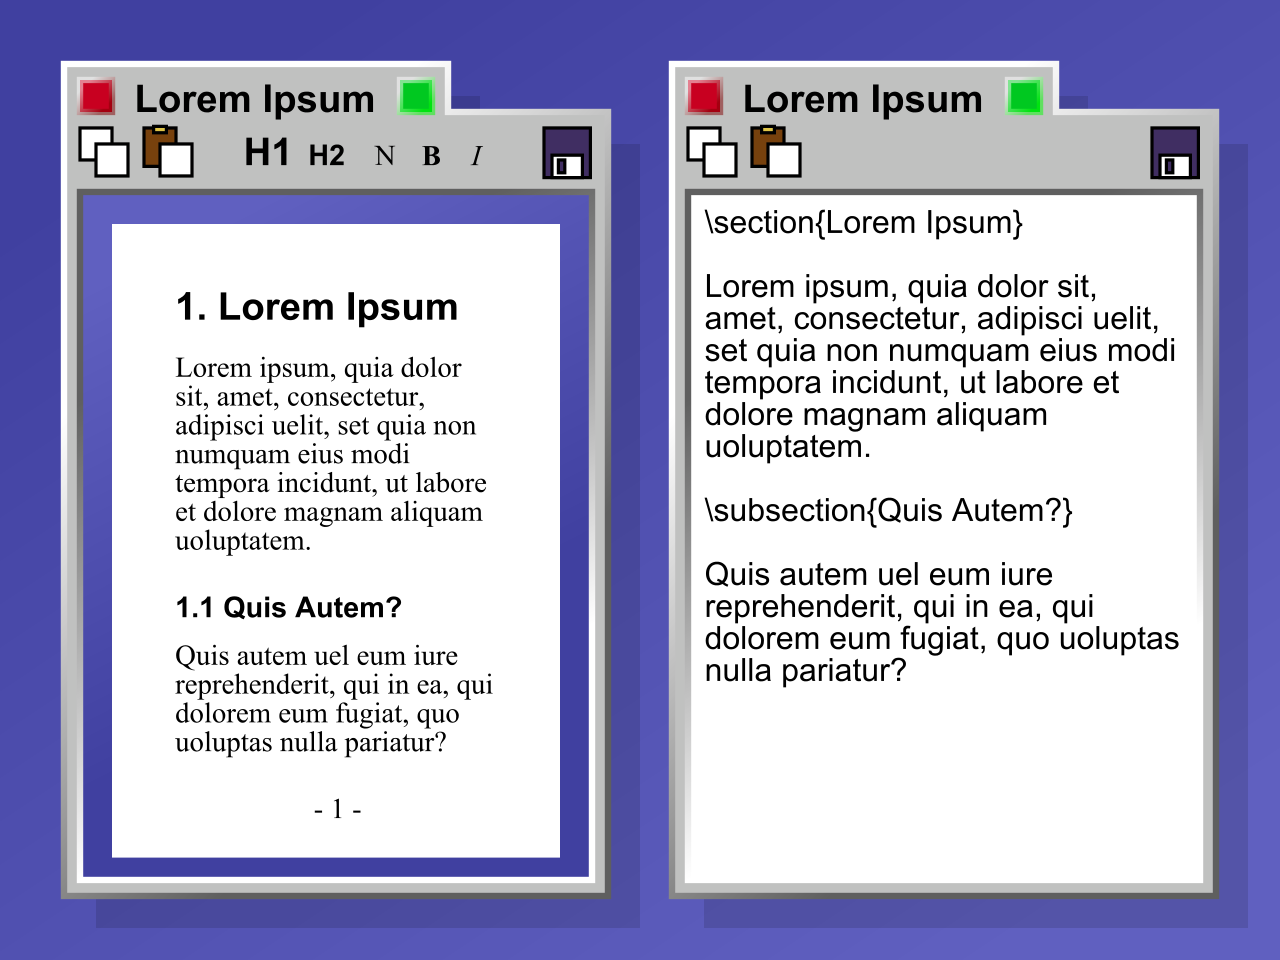
\includegraphics[width=\textwidth]{latex.png}
\end{frame}

\begin{frame}{Табличные процессоры}
  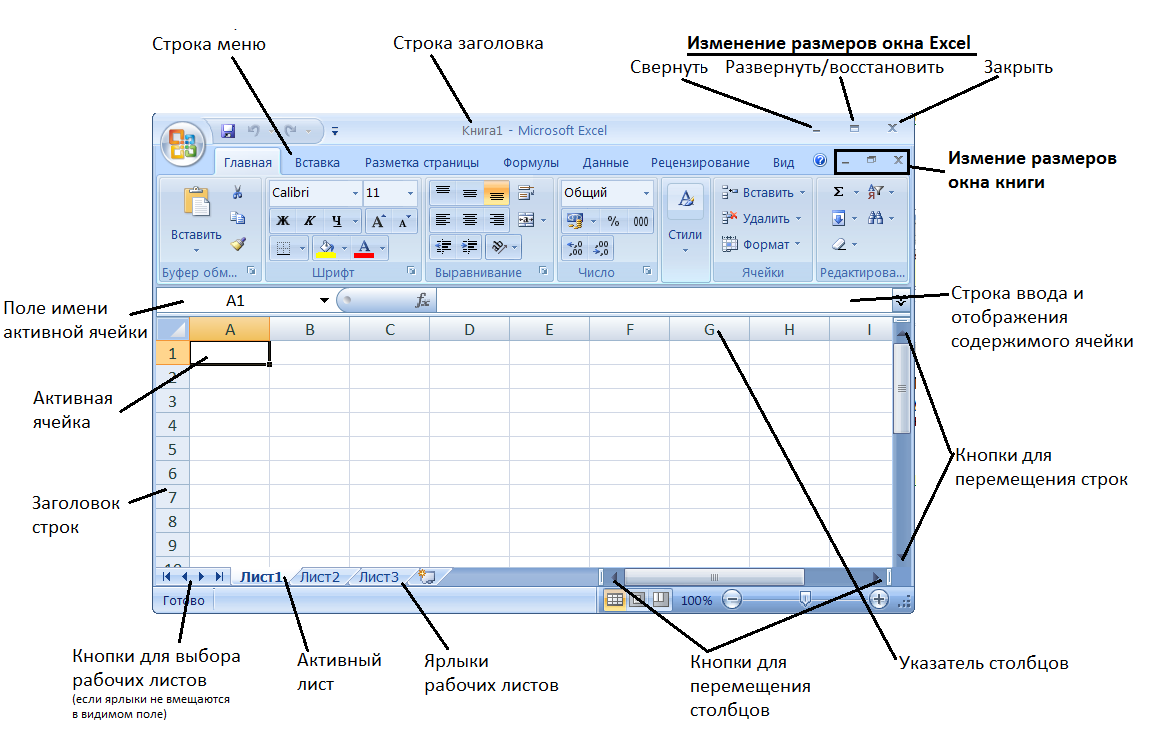
\includegraphics[width=\textwidth]{exel.png}
\end{frame}

\begin{frame}{Базы данных}
  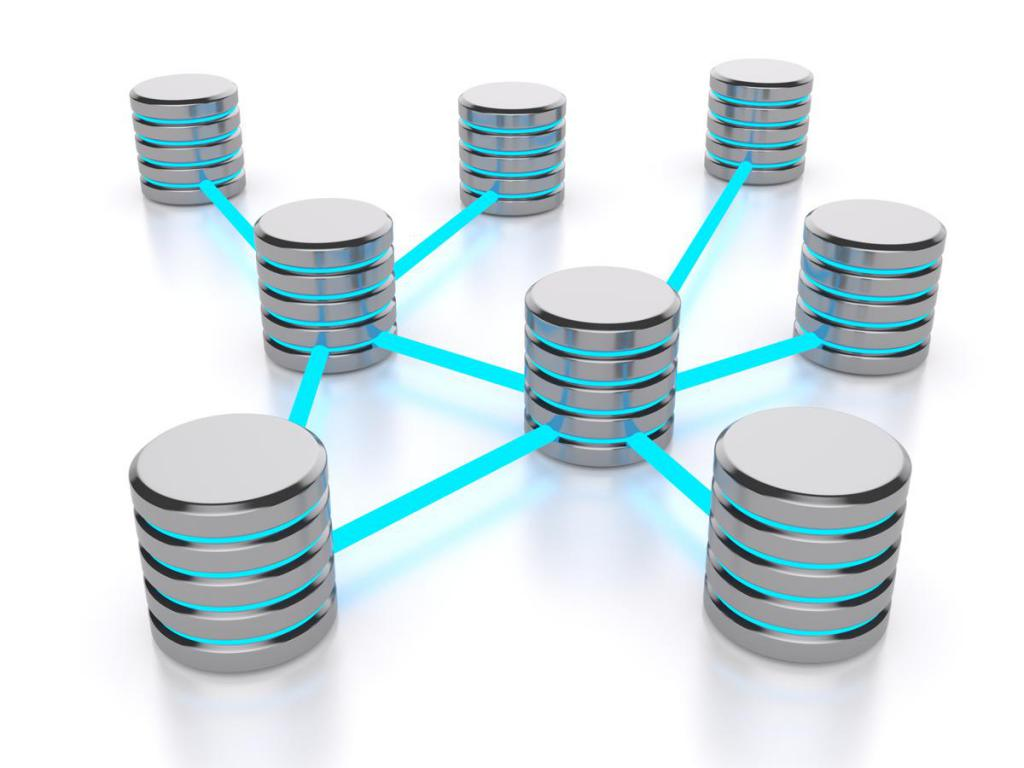
\includegraphics[width=\textwidth]{db.jpg}
\end{frame}

\begin{frame}{Реляционные базы данных}
  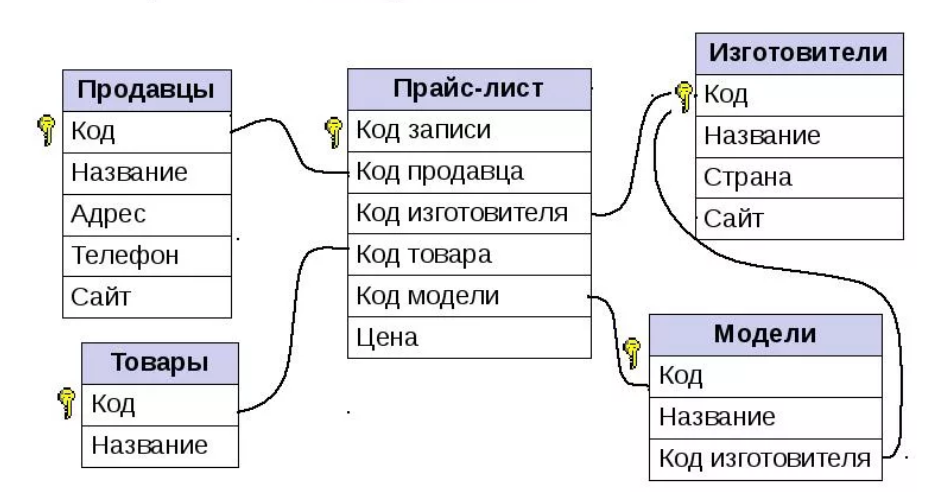
\includegraphics[width=\textwidth]{rdb.png}
\end{frame}

\end{document}
